\documentclass[8pt]{beamer}\usepackage[]{graphicx}\usepackage[]{color}


\usetheme{metropolis}           % Use metropolis theme
\usepackage{amsmath}
\usepackage{mathrsfs}
\usepackage{tabularx}
\usepackage{tikz}
\usetikzlibrary{patterns}

% For custom oversets
\usepackage{accents}


\usepackage[style=authoryear]{biblatex}
\addbibresource{references.bib}
\usepackage{cleveref}
\renewcommand*{\bibfont}{\footnotesize}


\def\coingrid{
\draw[step=1cm,gray,very thin] (0,0) grid (2,3);
\node[left, color=blue] at (0, 2.5) {Coin TT};
\node[left, color=blue] at (0, 1.5) {Coin HT};
\node[left, color=blue] at (0, 0.5) {Coin HH};
\node[above, color=purple] at (0.5, 3) {Side 1};
\node[above, color=purple] at (1.5, 3) {Side 2};
\node[below right, color=black] at (0, 3) {\tiny TT1};
\node[below right, color=black] at (0, 2) {\tiny HT1};
\node[below right, color=black] at (0, 1) {\tiny HH1};
\node[below right, color=black] at (1, 3) {\tiny TT2};
\node[below right, color=black] at (1, 2) {\tiny HT2};
\node[below right, color=black] at (1, 1) {\tiny HH2};
}

\def\rectfill#1#2#3#4{
\draw[pattern=#1, pattern color=#2] (#3,#4) rectangle (#3 + 1,#4 + 1);
}


\def\p#1{\mathbb{P}\left(#1\right)}
\def\q#1{\mathbb{Q}\left(#1\right)}
\def\y{y}
\def\z{z}
\def\normz{\mathcal{N}(z)}
\def\etahat{\hat{\eta}}
\def\ellhat{\hat{\ell}}
\def\sumn{\sum_{n=1}^N}
\def\meann{\frac{1}{N} \sumn}
\newcommand{\etastar}{\accentset{*}{\eta}}
\def\Z{\mathcal{Z}}
\def\expect#1#2{\mathbb{E}_{#1}\left[#2\right]}
\def\kl#1{\mathrm{KL}\left(#1\right)}
\def\klhat#1{\widehat{\mathrm{KL}}\left(#1\right)}
\def\ind#1{1\left(#1\right)}

\DeclareMathOperator*{\argmax}{\mathrm{argmax}}
\DeclareMathOperator*{\argmin}{\mathrm{argmin}}
\DeclareMathOperator*{\esssup}{\mathrm{esssup}}
\DeclareMathOperator*{\essinf}{\mathrm{essinf}}
\DeclareMathOperator*{\argsup}{\mathrm{argsup}}
\DeclareMathOperator*{\arginf}{\mathrm{arginf}}

\title{Inductive logic: Introduction and context}
\author{Ryan Giordano}
\date{Sep 23rd, 2022}
\institute{Massachusetts Institute of Technology}

\begin{document}




%%%%%%%%%%%%%%%%%%%%%%%%%%%%%%%%%%%%%%%%%%%%%%%%%%%%%%%%%%%%%%%%%%%%%%%
%%%%%%%%%%%%%%%%%%%%%%%%%%%%%%%%%%%%%%%%%%%%%%%%%%%%%%%%%%%%%%%%%%%%%%%
%%%%%%%%%%%%%%%%%%%%%%%%%%%%%%%%%%%%%%%%%%%%%%%%%%%%%%%%%%%%%%%%%%%%%%%

\begin{frame}{Outline}
%
\begin{itemize}
%
\item Logic
\item Deduction and induction
\item Classes of inductive questions (from philosophical induction to probability)
\item Extreme resolutions: ``Bayesian,'' ``falsificationist,'' ``conventionalist''
%
\end{itemize}
%
\end{frame}

%%%%%%%%%%%%%%%%%%%%%%%%%%%%%%%%%%%%%%%%%%%%%%%%%%%%%%%%%%%%%%%%%%%%%%%
%%%%%%%%%%%%%%%%%%%%%%%%%%%%%%%%%%%%%%%%%%%%%%%%%%%%%%%%%%%%%%%%%%%%%%%
%%%%%%%%%%%%%%%%%%%%%%%%%%%%%%%%%%%%%%%%%%%%%%%%%%%%%%%%%%%%%%%%%%%%%%%

\begin{frame}{Logic}
%
As far as we know, among the great ancient civilizations, only the Greeks
studied the formal validity of argumentation, a.k.a., logic
(\cite{shenefelt:2013:ifathenb}).  This presentation will borrow a lot from the
lucid and readable reference \cite{hacking:2001:introduction}.

\pause
Logic studies the {\em validity} of an argument, not the {\em truth} of
its conclusions.

An argument is valid if it is logically sound.

A proposition is a statement which is either true or false.

\vspace{1em}
\textbf{Example: }\\
If James wants a job, then he will get a haircut tomorrow.\\
James will get a haircut tomorrow.\\
So: James wants a job.

\vspace{1em}
If James wants a job, then he will get a haircut tomorrow.\\
James wants a job.\\
So: James will get a haircut tomorrow.

\pause
\vspace{1em}
\textbf{Questions:} \\
Which argument is valid?  \\
What are the propositions?\\
Which propositions are true?
%
\end{frame}



%%%%%%%%%%%%%%%%%%%%%%%%%%%%%%%%%%%%%%%%%%%%%%%%%%%%%%%%%%%%%%%%%%%%%%%
%%%%%%%%%%%%%%%%%%%%%%%%%%%%%%%%%%%%%%%%%%%%%%%%%%%%%%%%%%%%%%%%%%%%%%%
%%%%%%%%%%%%%%%%%%%%%%%%%%%%%%%%%%%%%%%%%%%%%%%%%%%%%%%%%%%%%%%%%%%%%%%

\begin{frame}{Logic}
%
\textbf{Which of these arguments are valid?}
(\cite[Ch.1 Question 7]{hacking:2001:introduction})

%
\begin{itemize}
%
\item I follow three major league teams.  Most of their top hitters chew
tobacco at the plate.\\
$\Rightarrow$ Chewing tobacco improves batting average.
%
\item The top six hitters in the National League chew tobacco at the plate.\\
$\Rightarrow$ Chewing tobacco improves batting average.
%
\item A study by the American Dental Association of 158 players on
seven major league teams during the 1988 season showed that the mean batting
average for chewers was 0.238 compared to 0.248 for non-users.  Abstainers
also had a higher fielding average.\\
$\Rightarrow$ Chewing tobacco does not improve batting average.
%
\item In 1921, every major league pitcher who chewed tobacco when up to
bat had a higher batting average than any major league pitcher who did
not.\\
$\Rightarrow$ Chewing tobacco does not improve batting average.
%
\end{itemize}
%
\pause
\textbf{None of them are valid.}

But some are better than others.
In what sense?  In any logical sense?
%
\end{frame}


%%%%%%%%%%%%%%%%%%%%%%%%%%%%%%%%%%%%%%%%%%%%%%%%%%%%%%%%%%%%%%%%%%%%%%%
%%%%%%%%%%%%%%%%%%%%%%%%%%%%%%%%%%%%%%%%%%%%%%%%%%%%%%%%%%%%%%%%%%%%%%%
%%%%%%%%%%%%%%%%%%%%%%%%%%%%%%%%%%%%%%%%%%%%%%%%%%%%%%%%%%%%%%%%%%%%%%%

\begin{frame}{Logic}

% Aristotle identified four ``categorical propositions'' that form the basis
% of his logic:
%
% %
% \begin{itemize}
% %
% \item All As are Bs.
% \item No As are Bs.
% \item Some As are Bs.
% \item Some As are not Bs.
% %
% \end{itemize}
% %
The Stoics identify the following syllogisms, purported patterns of
valid inference:
%
\begin{itemize}
%
\item \emph{Modus Ponens}: If A, then B.  A.  Therefore, B.
\item \emph{Modus Tollens}: If A, then B.  Not B.  Therefore, not A.
\item The Hypothetical Syllogism: If A, then B.  If B, then C.  Therefore, if A, then C.
\item The Conjunctive Syllogism: Not both A and B.  A.  Therefore, not B.
\item The Dilemma: If A, then B.  If C, then B.  A or C.  Therefore, B.
\item The Disjunctive Syllogism: A or B.  But not A.  Therefore, B.
%
\end{itemize}
%
All logic consists of identifying rules like these which, when applied to
true premises, guarantees true conclusions.

Humans are free to construct ``logics,'' which may
or may not actually produce something we are willing to call truth.  To
paraphrase \cite{hacking:2016:logic}:

\begin{block}{}
%
``The problem of the [logic] is to state a set of principles
which entail the validity of all correct [inference], and which do not
imply that any fallacious inference is valid.''
%
\end{block}
%
\end{frame}


%%%%%%%%%%%%%%%%%%%%%%%%%%%%%%%%%%%%%%%%%%%%%%%%%%%%%%%%%%%%%%%%%%%%%%%
%%%%%%%%%%%%%%%%%%%%%%%%%%%%%%%%%%%%%%%%%%%%%%%%%%%%%%%%%%%%%%%%%%%%%%%
%%%%%%%%%%%%%%%%%%%%%%%%%%%%%%%%%%%%%%%%%%%%%%%%%%%%%%%%%%%%%%%%%%%%%%%


\begin{frame}{Example}
%
Set theory can provide a means to visualize and analyze logical reasoning.
Here is an example that I think may be useful.\footnote{I cooked this up and
have no idea how standard this is.  I realized preparing for this how
little I know about logic.}


Suppose a bag contains three coins: one regular coin (HT), one with both
faces tails (TT), and one with both faces heads (HH).  The coin is flipped,
and either the first or second side comes up.

Exactly one possible outcome
of coin $\times$ side occurs; call this the ``truth.''

\begin{minipage}{0.38\textwidth}
    \begin{center}
    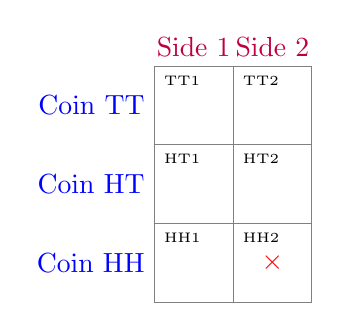
\begin{tikzpicture}
        \coingrid{}
        \node[color=red] at (1.5, 0.5) {$\times$};
    \end{tikzpicture}
\end{center}
\end{minipage}
\begin{minipage}{0.58\textwidth}
    %
    \textbf{Example:}\\
    Coin HH was picked and the second side came up (HH2).

    \vspace{1em} In this context, classical propositional logic can be
    represented as set operations.
    %
\end{minipage}
%
\end{frame}

%%%%%%%%%%%%%%%%%%%%%%%%%%%%%%%%%%%%%%%%%%%%%%%%%%%%%%%%%%%%%%%%%%%%%%%
%%%%%%%%%%%%%%%%%%%%%%%%%%%%%%%%%%%%%%%%%%%%%%%%%%%%%%%%%%%%%%%%%%%%%%%
%%%%%%%%%%%%%%%%%%%%%%%%%%%%%%%%%%%%%%%%%%%%%%%%%%%%%%%%%%%%%%%%%%%%%%%

\begin{frame}{Example}

\begin{minipage}{0.38\textwidth}
    \begin{center}
    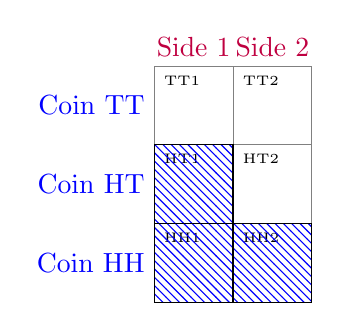
\begin{tikzpicture}
        \coingrid{}
        \rectfill{north west lines}{blue}{0}{0}
        \rectfill{north west lines}{blue}{0}{1}
        \rectfill{north west lines}{blue}{1}{0}
    \end{tikzpicture}
\end{center}
\end{minipage}
\begin{minipage}{0.58\textwidth}
    %
    \vspace{1em} In this context, classical propositional logic can be
    represented as set operations.
    %
\end{minipage}

\end{frame}


%%%%%%%%%%%%%%%%%%%%%%%%%%%%%%%%%%%%%%%%%%%%%%%%%%%%%%%%%%%%%%%%%%%%%%%
%%%%%%%%%%%%%%%%%%%%%%%%%%%%%%%%%%%%%%%%%%%%%%%%%%%%%%%%%%%%%%%%%%%%%%%
%%%%%%%%%%%%%%%%%%%%%%%%%%%%%%%%%%%%%%%%%%%%%%%%%%%%%%%%%%%%%%%%%%%%%%%

\begin{frame}{Bibliography}
\printbibliography{}
\end{frame}

\end{document}
